\chapter{Results, usage and future work} 

\label{Chapter7} 

\lhead{Chapter 7. \emph{Results, usage and future work}}

\section{Performance}
\label{sec:performanceanalysis}
Performance has been the main concern in the development of the system. As already seen in previous chapters, many efforts have been made in order to achieve a good responsiveness to user input in the real time application. We made the clear choice of preferring low times in the offline computation of descriptors (reported in Table~\ref{table:benchmarkoffline}) for this has helped us in achieving good response times in the real time application. The latter ones, in general, greatly vary with the use of the application. For instance, the user interaction with sliders has the effect of emptying the playlist queue (which will result in temporary shorter computational times, due to the use of the least precise but fastest music similarity computation algorithm in order to get some new element into the playlist as soon as possible), while choosing to use longer segments or not interacting with the sliders may increase the computational time (for the system realizes that it has more time available for computing music similarity and then uses the most accurate algorithm\footnote{We recall that the only difference between the two algorithms lies in the choice of the similarity function, as shown at the point 8 of Section~\ref{subsec:rtalgorithm}}). \\
In other words, we have built an \textit{adaptive} system, defined in \cite{stober11} as a system that:
\begin{itemize}
\item Behaves different in different contexts given the same input, and
\item Performs this adaptation in order to optimize the system's behaviour in the given context according to some predefined measure.
\end{itemize}
In order to analyze its performance, we decided to collect data about computational times of the real time application for the choice of 1000 consecutive excerpts, with occasional interaction of the user. This is a reasonable analysis case, for it may be very similar to the real use of the system and also provides a good perspective on the computational times while using the most demanding algorithm of the system for computing music similarity. The hardware used in this analysis is the one reported in Table~\ref{table:hardwareoffline}. The results are shown for each main point of the procedure explained in Section~\ref{subsec:rtalgorithm}.\\

\begin{figure}[h]
\begin{center}
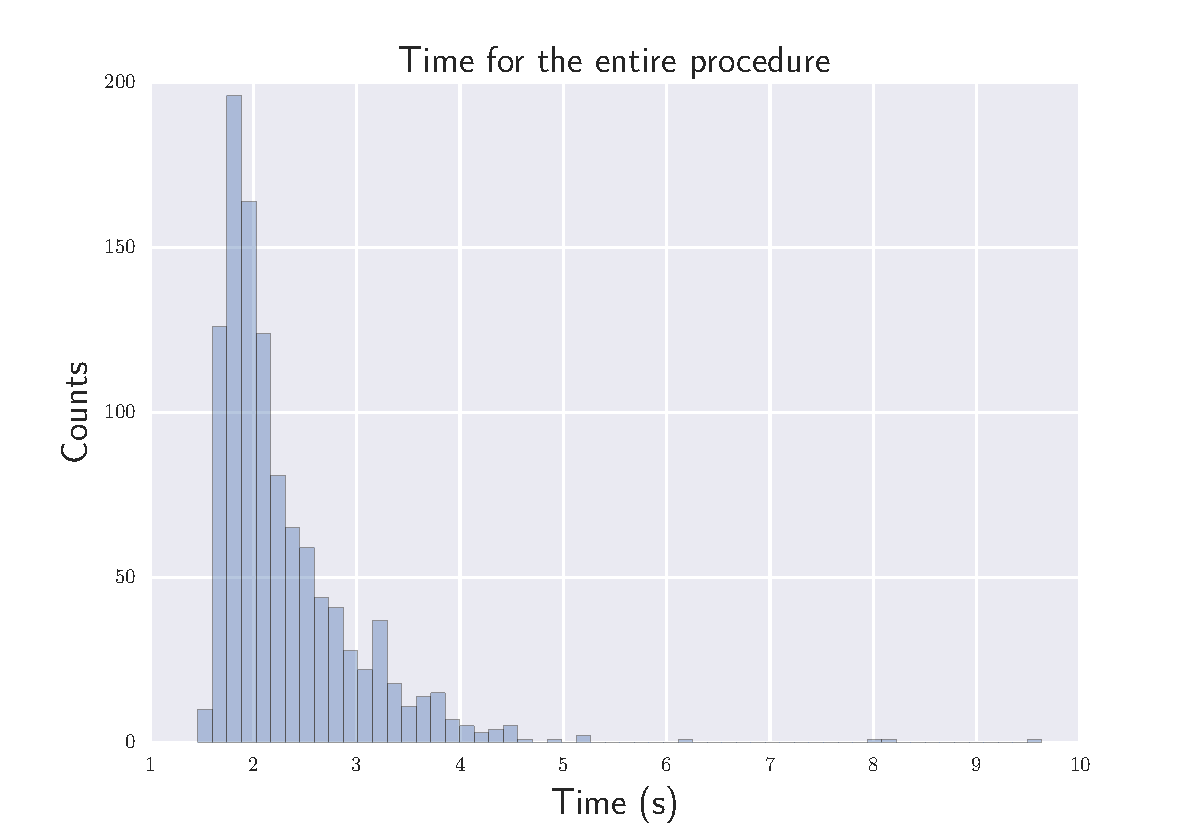
\includegraphics[scale=0.7]{Figures/bench_procedure.pdf}
    % \rule{10em}{0.5pt}
  \caption[Global time for selecting next segment]{Global time for selecting next segment.}
  \label{fig:step7}
\end{center}
\end{figure}

It can be seen that most of the times, the algorithm for choosing the next excerpt requires between 1.5 seconds and 3 seconds. The presence of some outliers above 5 seconds is due to particular conditions of the environment or of the operative system (such as some other process starting running in the background) and should not be considered meaningful for judging the performance of the algorithm itself. \\
We consider particurly appreciable that the system is capable of adapting its responsiveness to the environment, while still getting good response times also with most intensive computations. As already stated, during this  experiment user interactions were occasional, leading the system to use the most intensive variant of the algorithm 732 out of 1000 times.\\ \\ 

\begin{figure}[htbp]
\begin{center}
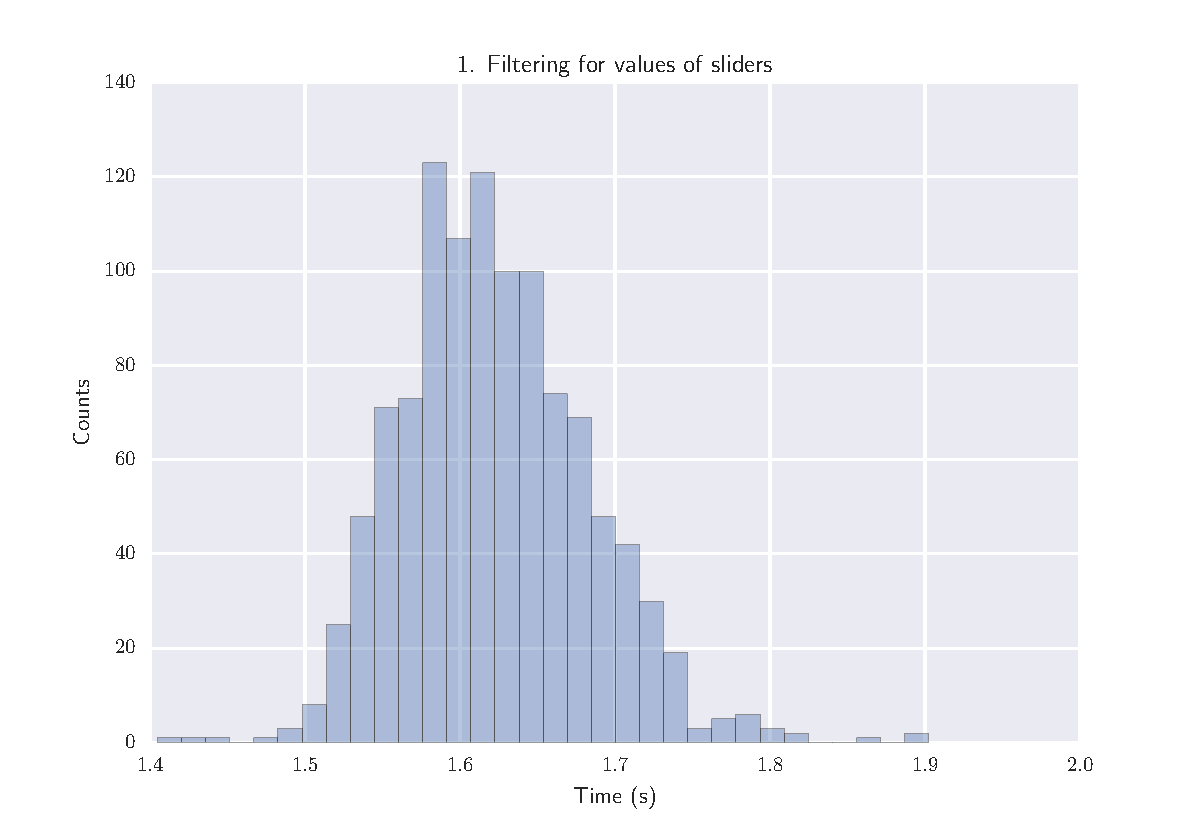
\includegraphics[scale=0.7]{Figures/bench_sliders.pdf}
    % \rule{10em}{0.5pt}
  \caption[Time for filtering music in regards to sliders' positions]{Time for performing the first step of the procedure: filtering of excerpts based on the current positions of sliders.}
  \label{fig:step1}
\vspace{2cm}
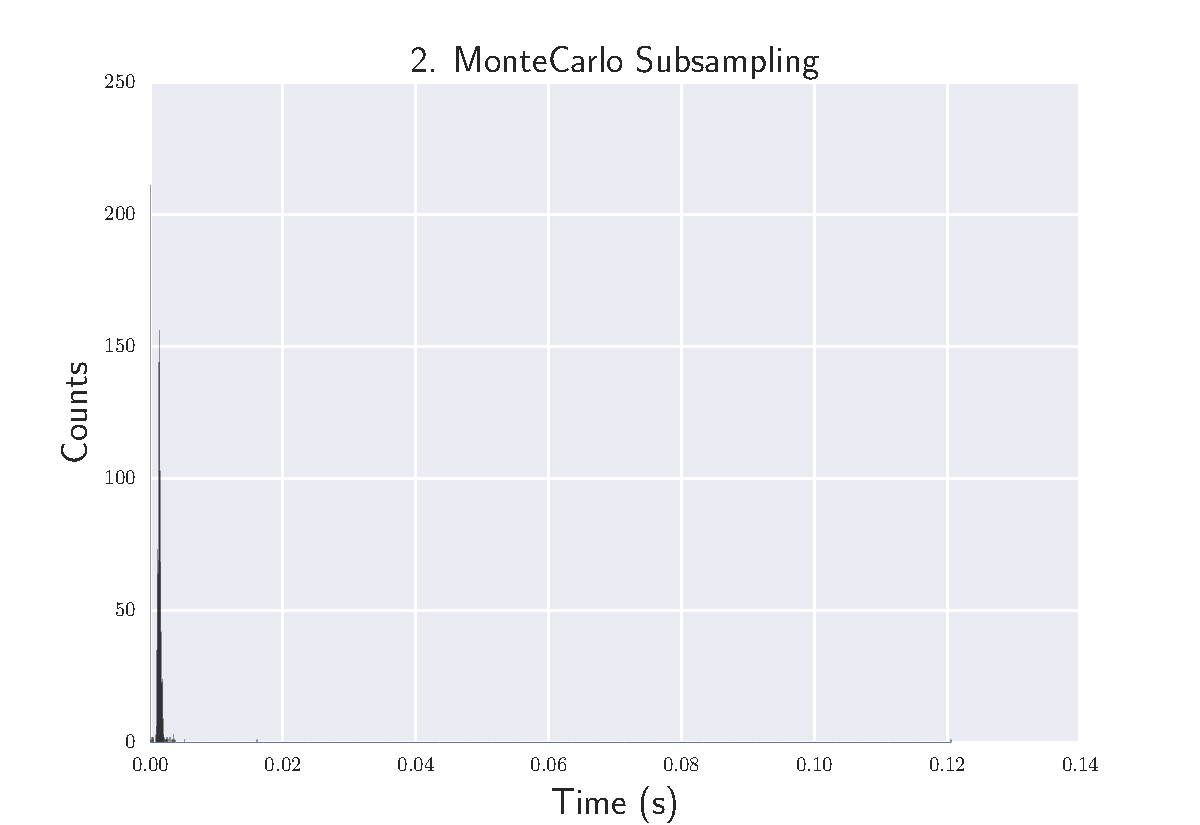
\includegraphics[scale=0.7]{Figures/bench_subsampling.pdf}
    % \rule{10em}{0.5pt}
  \caption[Time for performing Monte Carlo sampling]{Time for performing Monte Carlo sampling.}
  \label{fig:step2}
\end{center}
\end{figure}

\begin{figure}[htbp]
\begin{center}
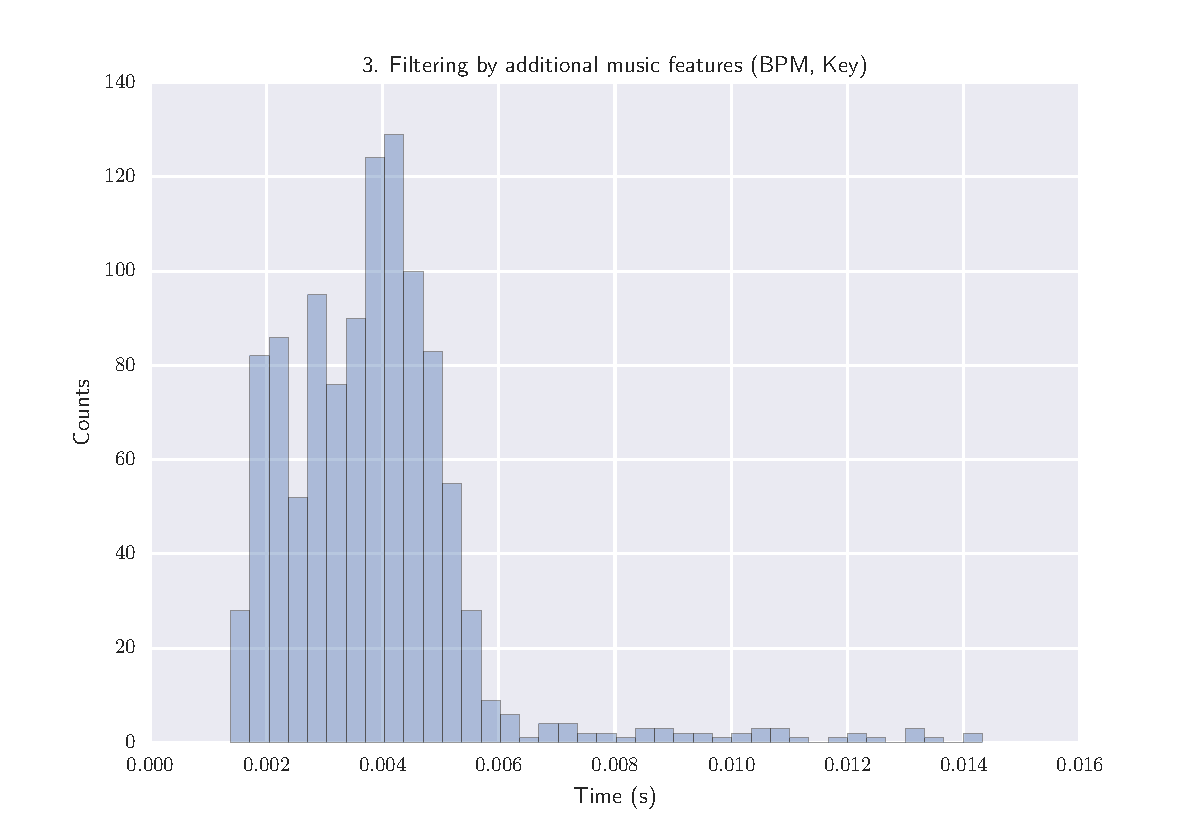
\includegraphics[scale=0.7]{Figures/bench_bpm_filters.pdf}
    % \rule{10em}{0.5pt}
  \caption[Time for filtering music according to musicality with current excerpt]{Time for filtering music according to musicality with current excerpt (in regards of BPM and key).}
  \label{fig:step3}
\vspace{2cm}
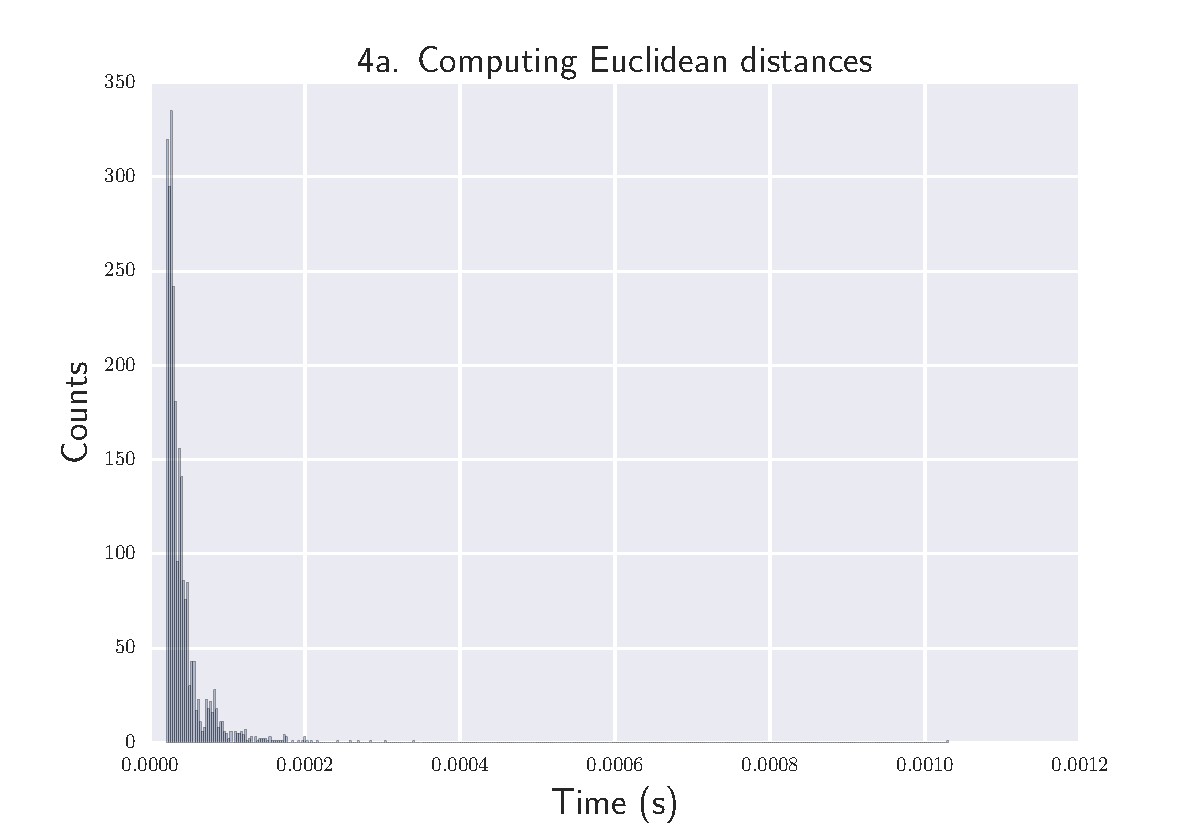
\includegraphics[scale=0.7]{Figures/bench_euclidean.pdf}
    % \rule{10em}{0.5pt}
  \caption[Time for computing euclidean distance]{Time for computing euclidean distance between two 20D points.}
  \label{fig:step4}
\end{center}
\end{figure}

\begin{figure}[htbp]
\begin{center}
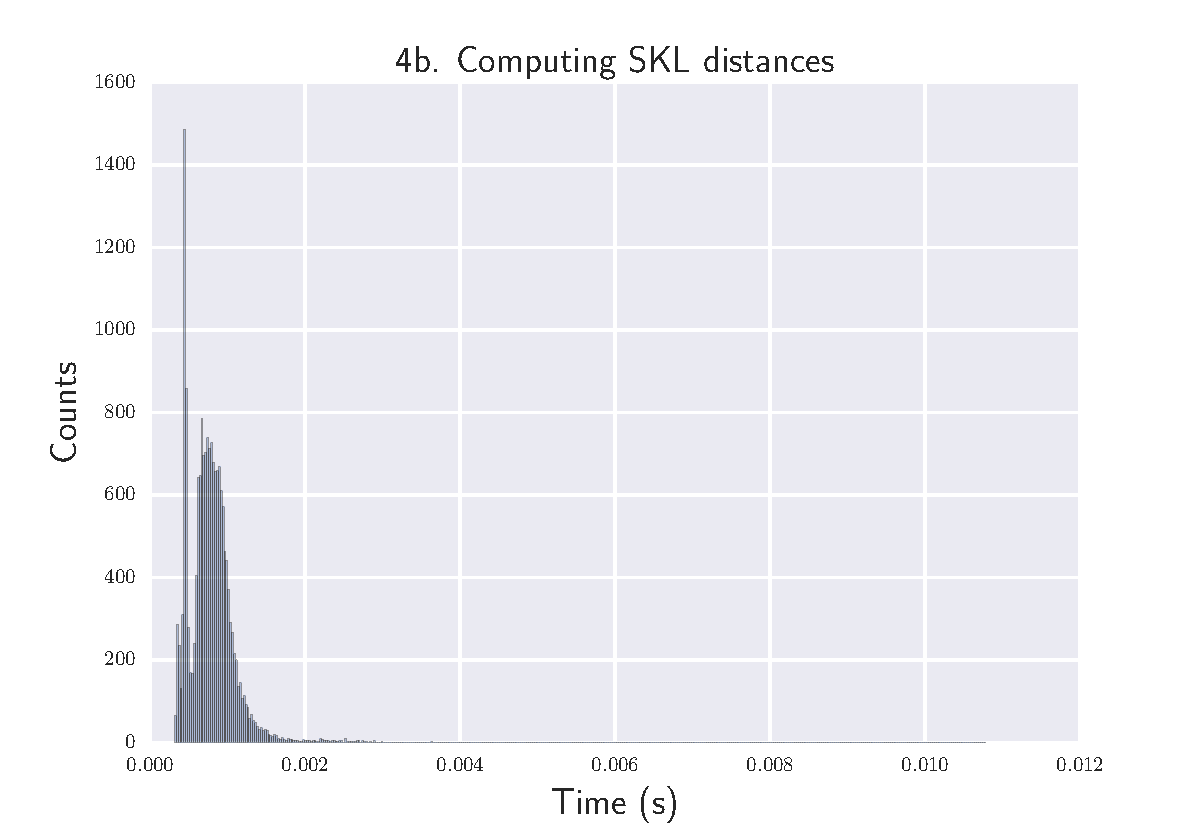
\includegraphics[scale=0.7]{Figures/bench_skl.pdf}
    % \rule{10em}{0.5pt}
  \caption[Time for computing symmetric Kullback-Leibler distance]{Time for computing symmetric Kullback-Leibler distance between two excerpts.}
  \label{fig:step5}
\vspace{2cm}
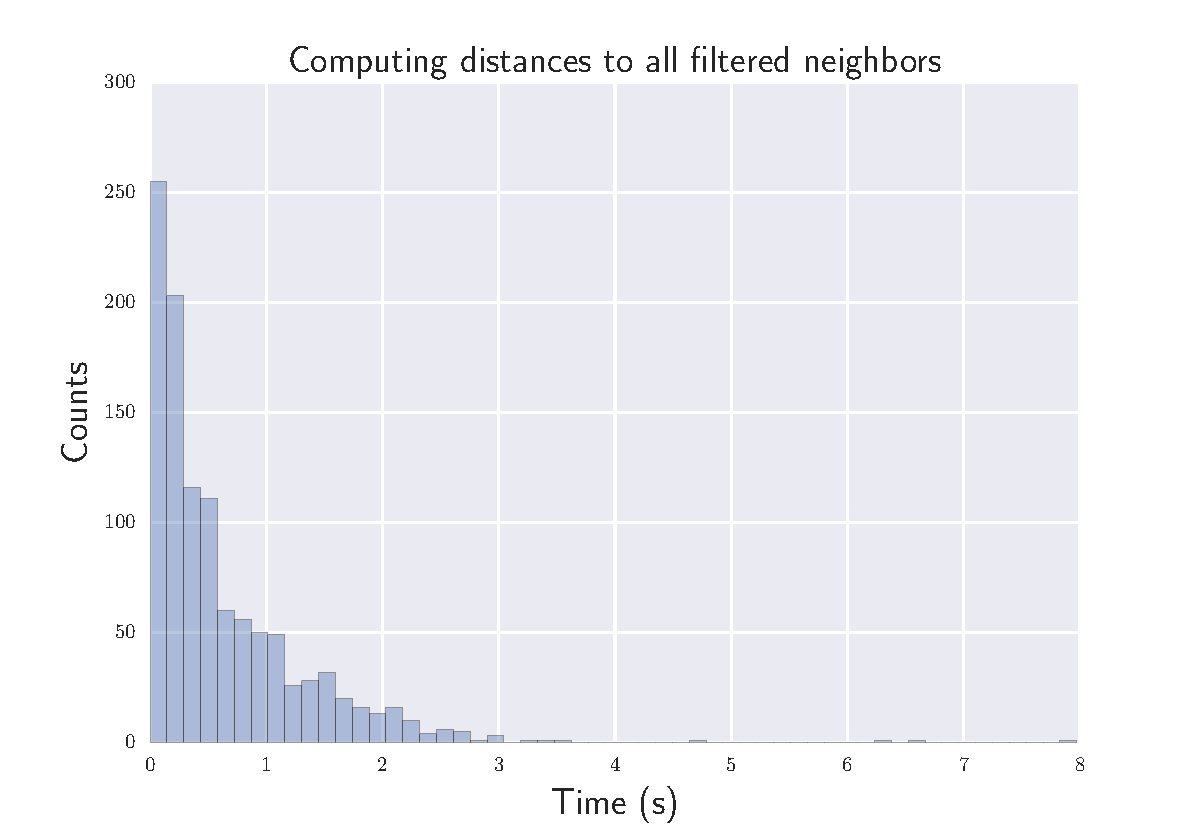
\includegraphics[scale=0.7]{Figures/bench_get_suitsegm.pdf}
    % \rule{10em}{0.5pt}
  \caption[Time for computing distances from all filtered segments]{Time for computing distances from all filtered segments.}
  \label{fig:step6}
\end{center}
\end{figure}

\begin{figure}[htbp]
\begin{center}
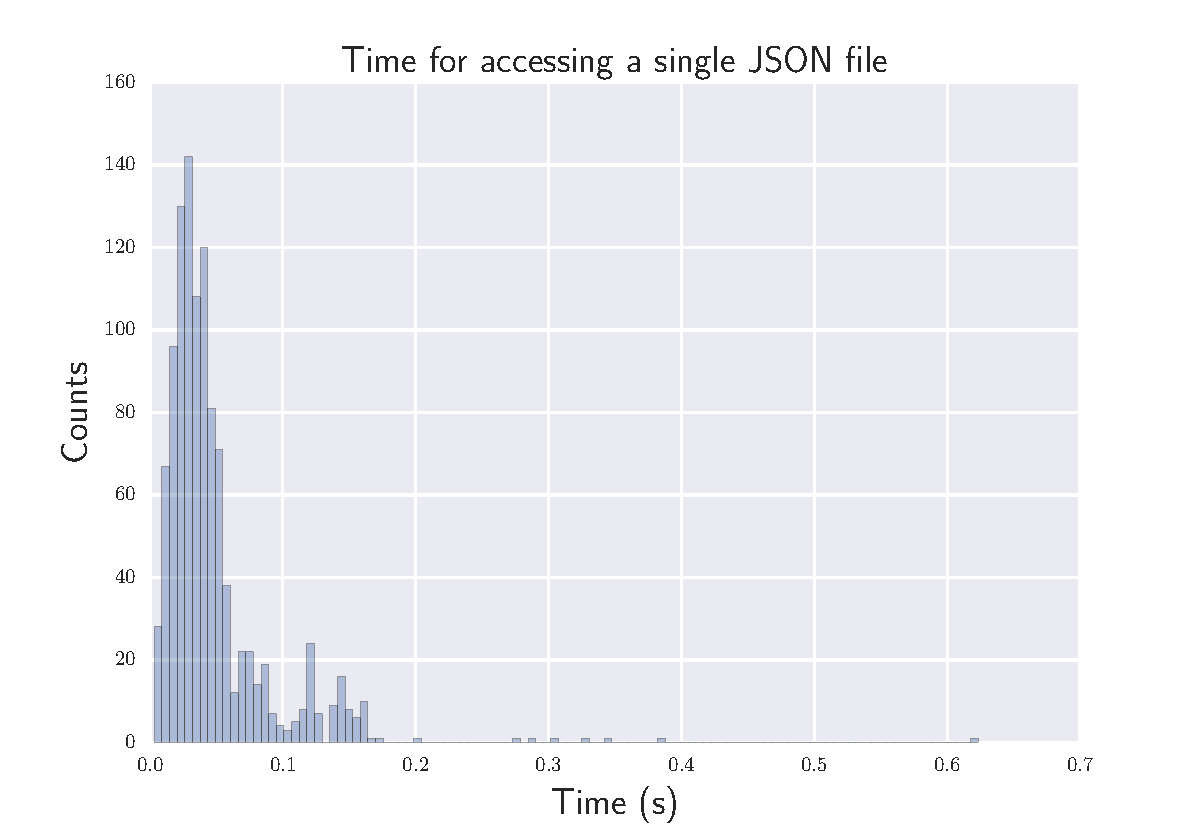
\includegraphics[scale=0.7]{Figures/bench_json_single.pdf}
    % \rule{10em}{0.5pt}
  \caption[Time for accessing and parsing a JSON file]{Time for accessing and parsing a JSON file.}
  \label{fig:step8}
\end{center}
\end{figure}

Looking at these graphs, several details emerge:
\begin{itemize}
\item Without any doubt, the most demanding task is the filtering of candidates on the base of sliders value. This is due to the fact that this is step acting on the highest number of excerpts. This filtering is based on values that are stored on RAM and therefore is not sensibly slowed down by the time for accessing these values. 
\item Random sampling, having possibly to act on a very large collection of excerpt, is one of the longest tasks.
\item Once all the filtering steps are done, computing all the similarity distances generally requires around one second. 
\item Computing symmetric Kullback-Leibler distance is around 10 times slower then computing Euclidean distance.
\item Time for accessing and parsing JSON file is not negligible and is actually 100 times longer than computing the symmetric Kullback-Leibler distance.
\end{itemize}

\section{Evaluation}
\label{sec:eval_results}
As explained in Section~\ref{sec:evaluation_idea}, we have decided to perform the evaluation of the system with specific experiments, followed by the compilation of a survey.
Specifically, the experiments are organized as follows:
\begin{itemize}
\item The subject of the experiment is introduced to the purpose of the application, without explaining any details about the interaction or the functioning;
\item The subject is given 5 minutes to freely interact with the application (playing with the Phonos collection of music), asking for clarification about the use if necessary;
\item The subject is finally given the chance to ask about more the functioning of the system;
\item The subject compiles a survey with specific questions about ease of useness, enjoyment of musical output, familiarity with the music and with this kind of software, and any problems. 
\end{itemize}

NUM subjects took part to this evaluation, with the following global results: \\
GRAPHS AND DISCUSSION

\section{Usage at exhibition} 
The inauguration of the exhibition has been on December 18th 2014, at Museu de la Musica, Barcelona. Many people have interacted with the system in order to explore the Phonos catalogue of music. The system hasn't incurred in any problem. At the time of the writing (February 2015), it's still daily used by several visitors at the Museum. The interactive kiosk will be dismissed at the end of the exhibition, on late September 2015.\\

\begin{figure}[htbp]
\begin{center}
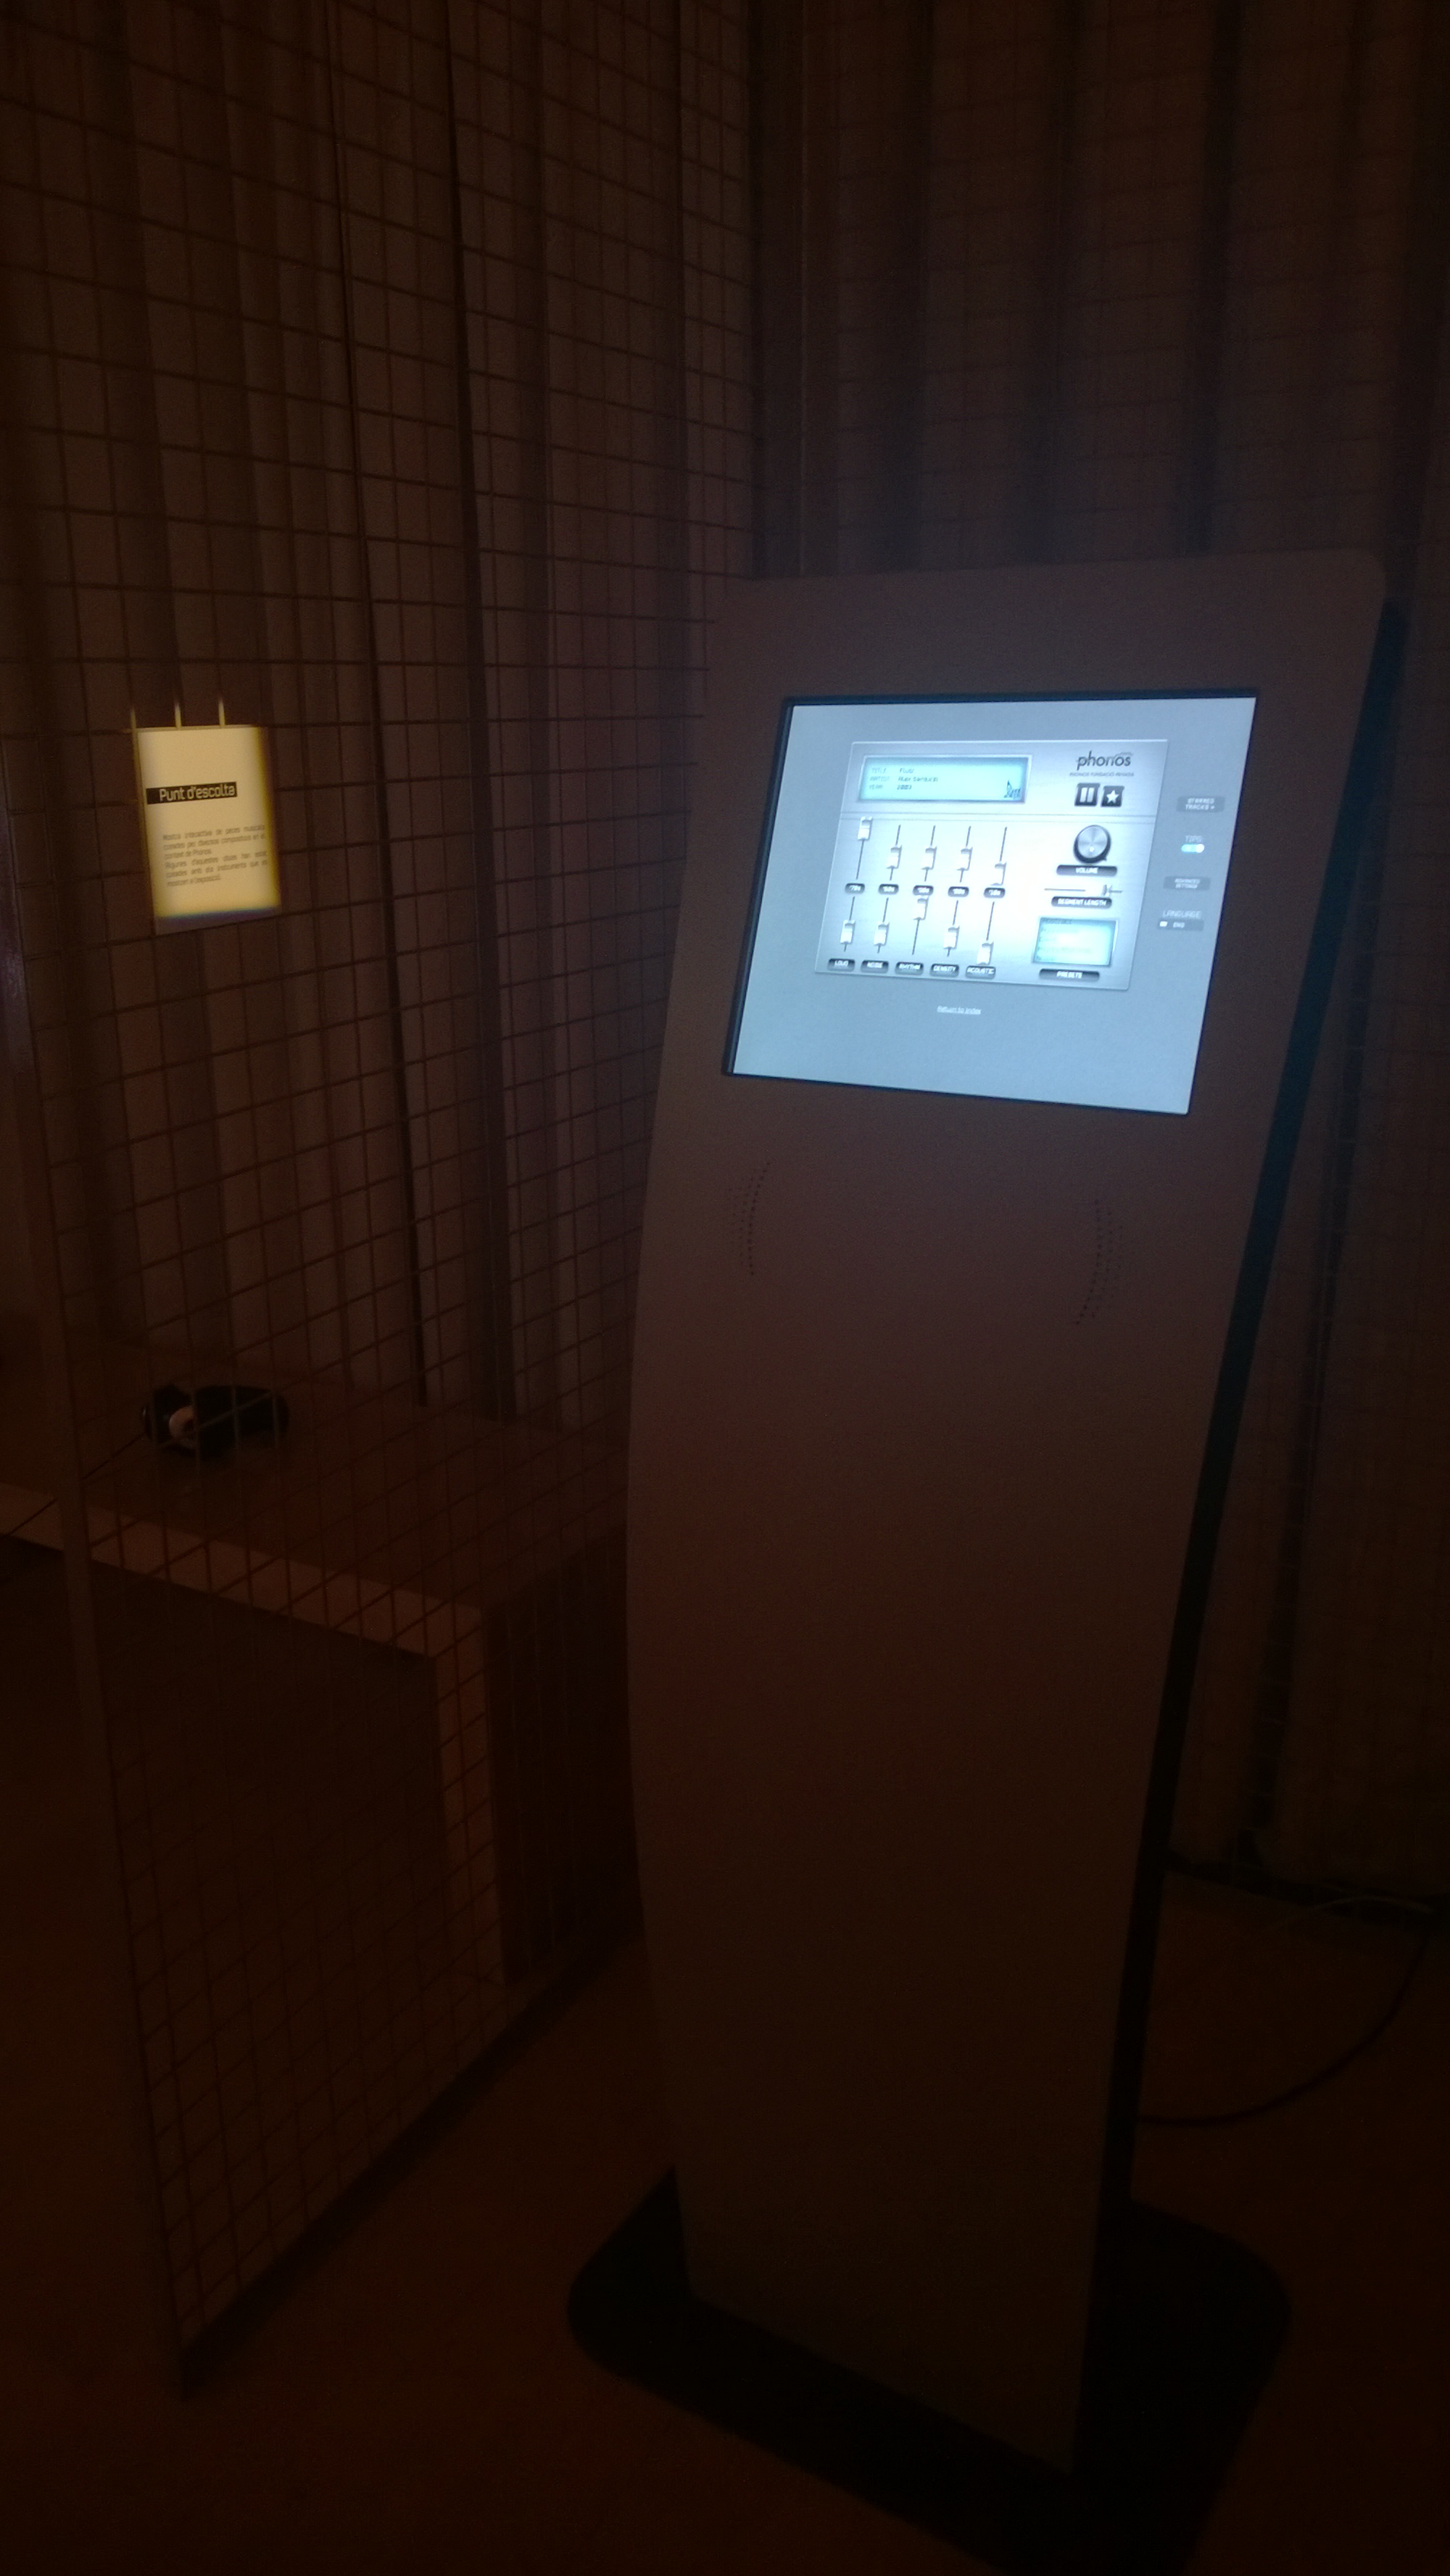
\includegraphics[scale=0.1]{Figures/kiosk1.jpg}

\vspace{1cm}

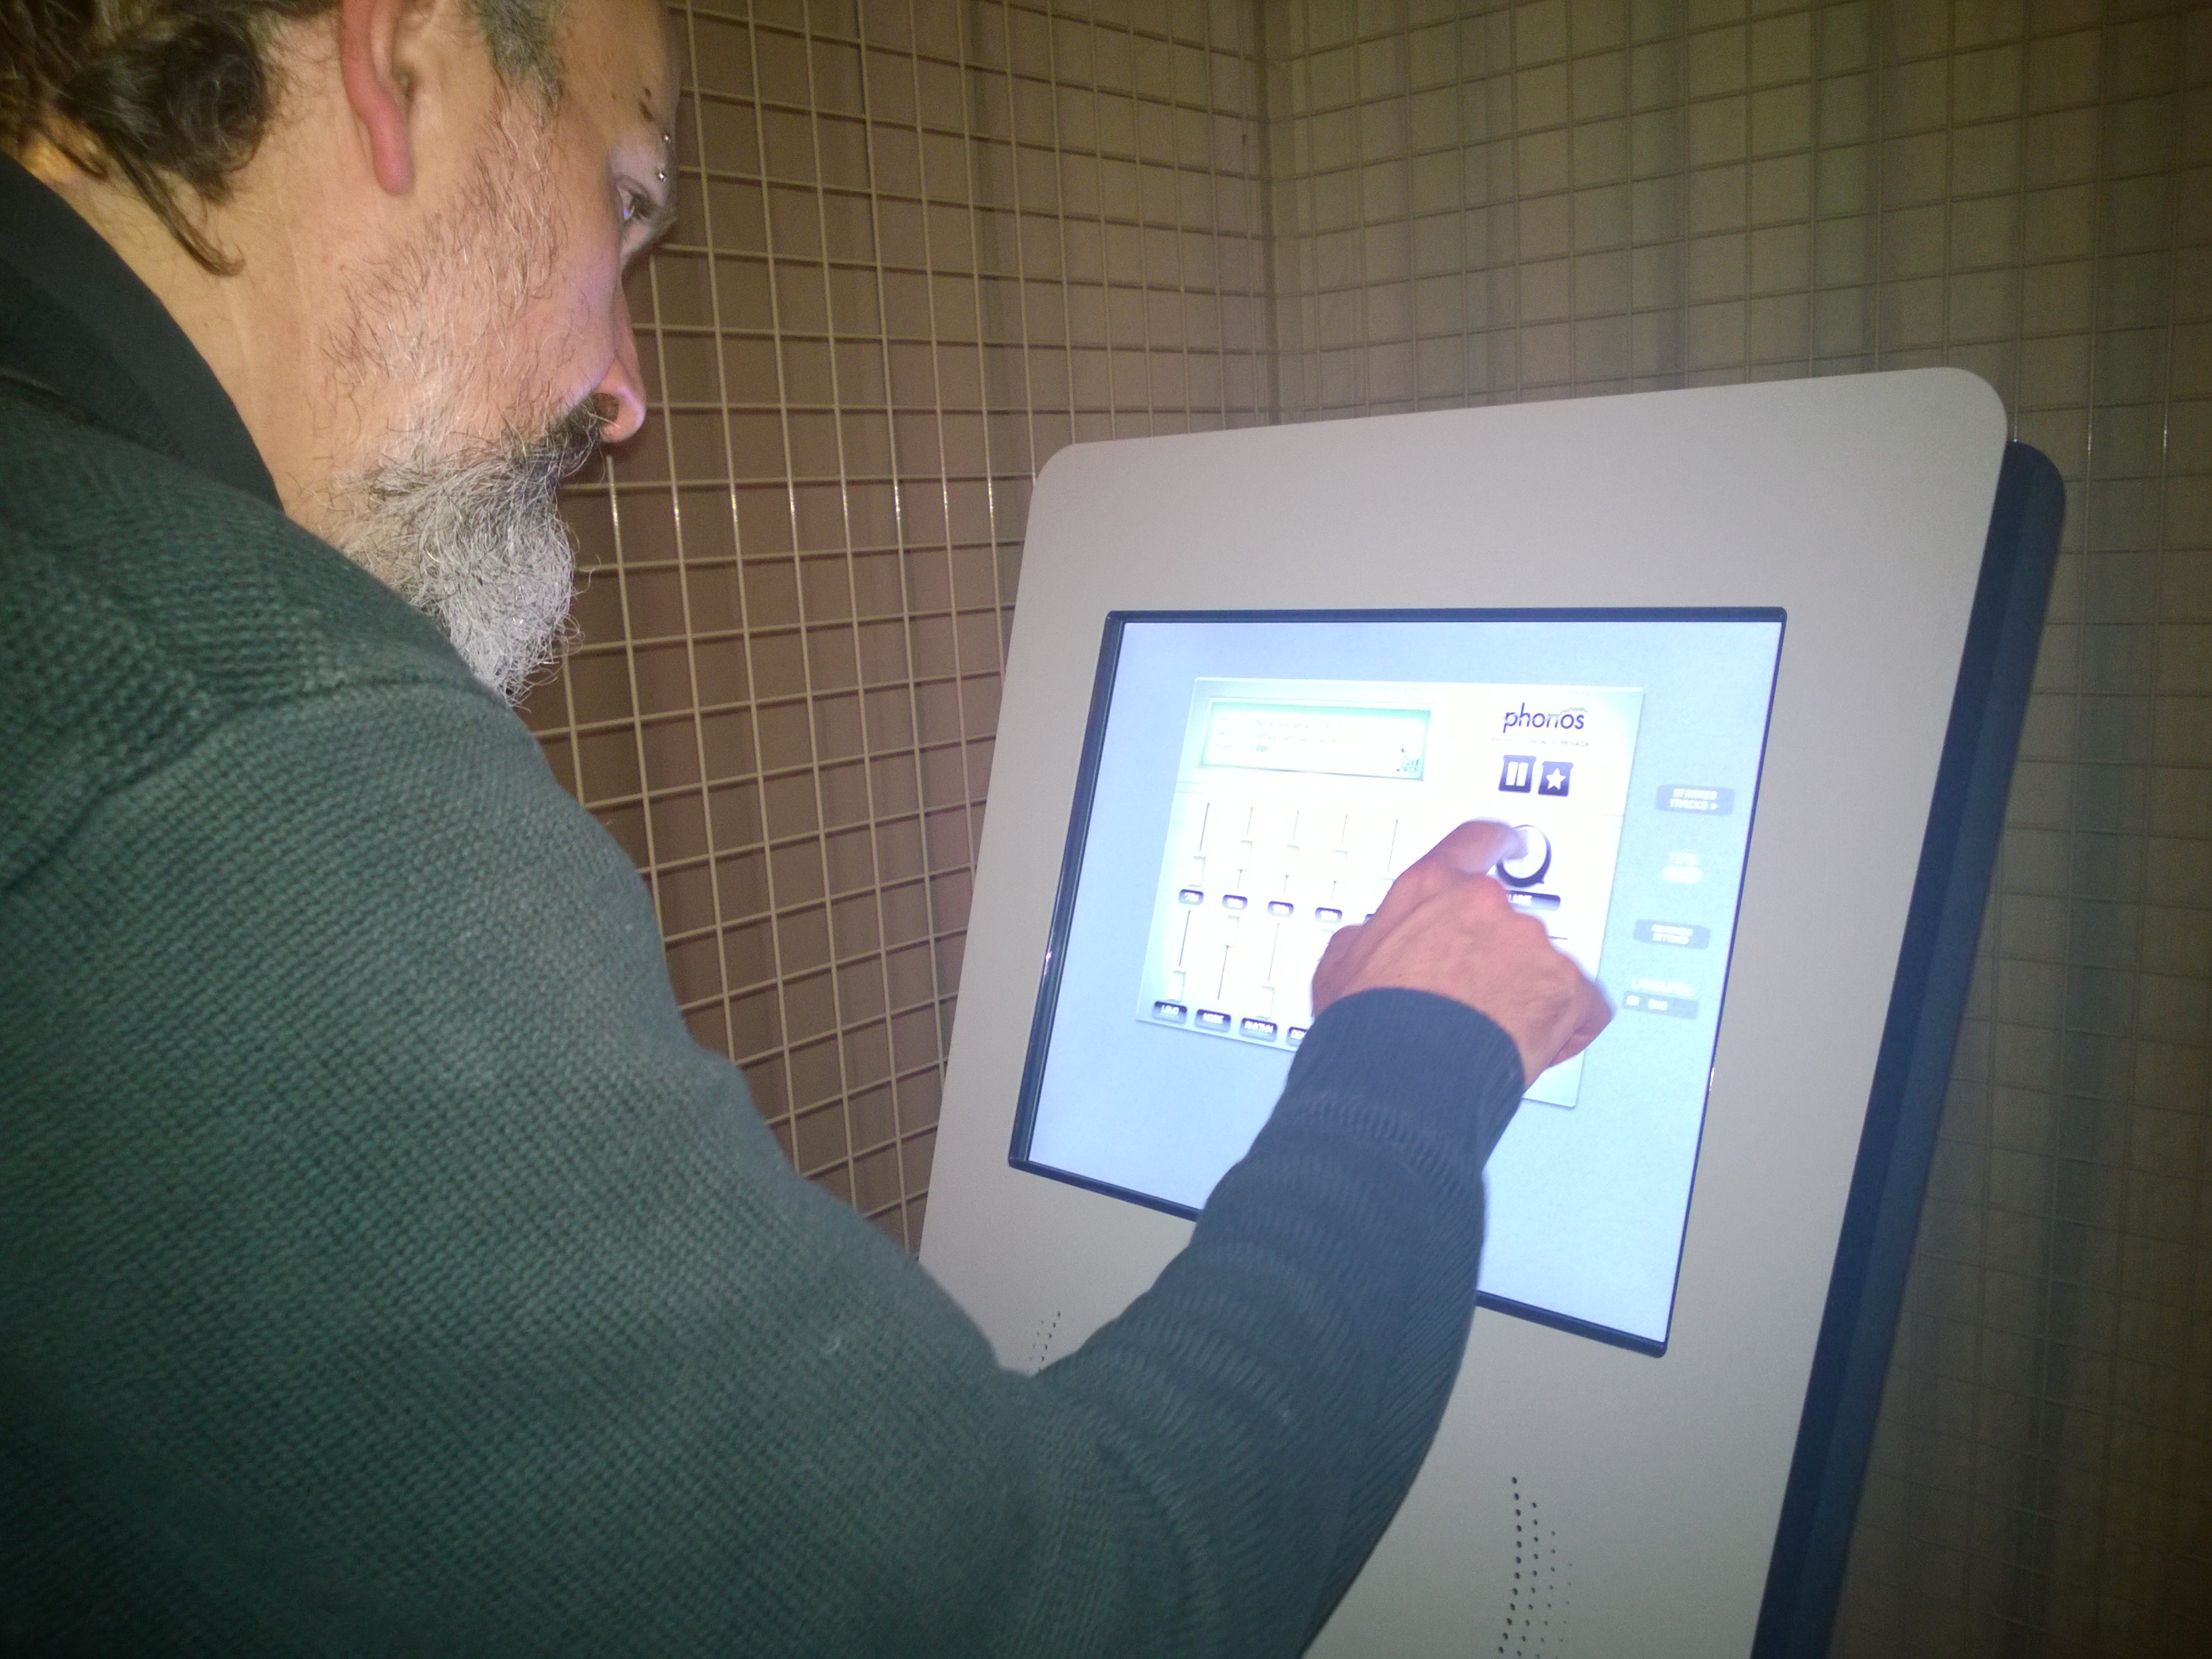
\includegraphics[scale=0.1]{Figures/kiosk2.jpg}
    \rule{20em}{0.5pt}
  \caption[Interactive kiosk at the exhibition]{Use of the interactive kiosk at the exhibition.}
  \label{fig:kiosk}
\end{center}
\end{figure}

\section{Results obtained by the study}
The main result achieved by the study was the exploitation of latest MIR findings for the development of a system that could easily be used by people not related to the research field and, more in general, not accustomed to the use of software. \\
This is a further proof that MIR technologies may be extremely useful in a wide range of applications, the most of which linked to common daily life situations. The software integrates not only different descriptors, but also different tools to extract them (Essentia and Echo Nest) in order to maximize the output, something that has rarely been done before.\\
Another contribute of this study lies in the integration of different researches into a single system: a study of of latest findings has been conducted in order to find what results have been achieved and could have been useful for our purposes. Despite being influenced by other solutions, ours constitutes an original way of solving the problem, for the algorithm we developed offer several new ideas; these are mainly due to the requirement of developing a low-latency system. Furthermore, the requirement of mixing together tracks (instead of just building a playlist of songs to be played one after another) has lead to the choice of implementing some personal musical knowledge in order to discard mixes that would have been perceived highly contrasting. This knowledge is especially related to the field of music composition and perception.\\

\section{Future work}
Despite having successfully reached its main goals, there is a lot of room for improving the system. \\
At first, the use of JSON files should be discarded in favour of much faster database tables, for instance PostgreSQL or MySQL. As seen in \ref{sec:performanceanalysis}, accessing and parsing JSON files is one of the slowest operations of the algorithm (almost 100 times longer than computing the symmetric Kullback-Leibler distance). Implementing a database should allow to use the more computationally intensive variant of the algorithm more frequently and to make the sampling less aggressive, therefore leading to generally better results. \\
The computation of music similarity could also be improved and use more sophisticated techniques, such as Fluctuation Patterns, that have shown very good results in similar systems \cite{pohle09}. \\
Furthermore, the development of a web application imposes several limitations (such as general low performances and high latency on audio streaming) that could easily be solved in a native mobile application for tablets or smartphones. \\
The source code for the application is entirely available at \url{https://github.com/giuband/Phonos-Music-Explorer}, so that many users can contribute in making it better.\\
Once the above cited aspects are refined, the development of the system could follow two different paths.
\begin{enumerate}
\item The system could be improved in its use for music discovery. For instance the user interface could implement some way of letting the user explore his current position inside the map of excerpts, in order to give a more clear idea about the music of the catalogue. New descriptors could be used and some of them could also be inherited from metadata or machine learning processes. 
\item The system could additionaly be integrated into a more creative environment for making music. It could be used for the automatic generation of recommendations while in the process of composing music. For instance, it could suggest the user of using a particular excerpt at some point of his composition to improve the quality of the work. It could also be used as the only source to compose music, providing the ability of automatically composing music made of excerpts while the user gives a direction to this flow, according to his creative intent. 
\end{enumerate}
The use suggested in 2. is particularly interesting, for such an application would perfectly fit the vision embraced by the GiantSteps project and provide a new system of producing music, making this amazing creative task accessible at anyone, indipendently from the skill. The process of making music could therefore overthrow its innate boundaries, leading to a world where the creation of art arises from the purest intent of contributing to the world cultural heritage, in spite of lack of limited technical knowledge, economic unavailability and physical impediments.